\begin{figure}[!htb]
    \centering
    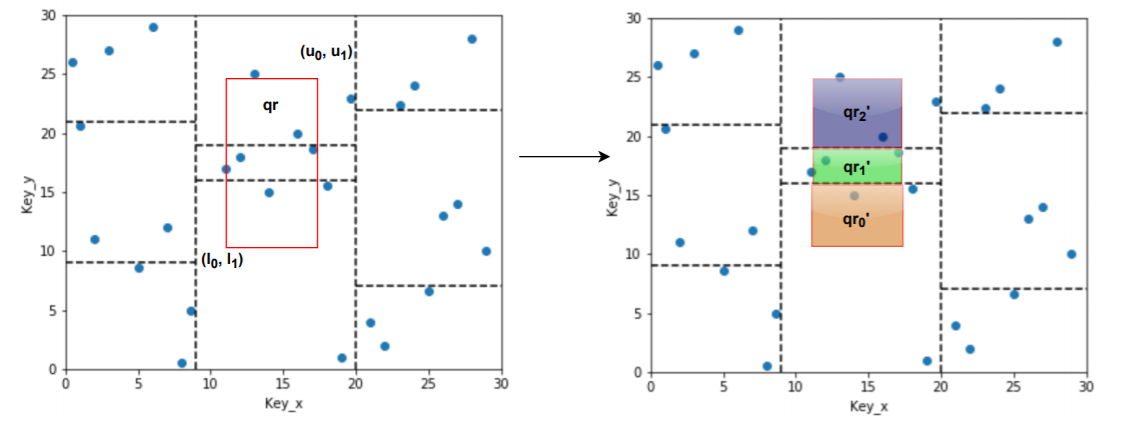
\includegraphics[width=\textwidth]{graphs/range_query_lisa.png}
    \caption{Range Query Search in Lisa}
    \label{fig:Range_Query_Lisa}
\end{figure}

For a range query $\mathcal{Q}(\boldsymbol{l},\boldsymbol{u})$, we first find the cells that overlap with $\mathcal{Q}$. Then we decompose $\mathcal{Q}$ into the union of smaller query rectangles $\bigcup \mathcal{Q}_i$ such that each smaller query rectangles intersects only one cell, as shown in the Fig. \ref{fig:Range_Query_Lisa}.

 Suppose that $\mathcal{Q}=\bigcup \mathcal{Q}_i$ where $\mathcal{Q}_i=[l_{i_0}, u_{i_o})\times [l_{i_1}, u_{i_1})$, i.e. we have $\mathcal{Q}_i$ representing the $i$th smaller query rectangles of one cell $C_j$.
 
 Then we can calculate the mapped values of $\mathcal{Q}_i$, i.e. $\mathcal{M}(l_{i_0}, l_{i_1})$ and $\mathcal{M}(u_{i_0}, u_{i_1})$. For simplicity, we use $m_l^{(i)}$ and $m_u^{(i)}$ to denote $\mathcal{M}(l_{i_0}, l_{i_1})$ and $\mathcal{M}(u_{i_0}, u_{i_1})$ respectively.
 
After creating corresponding mapped values, we then apply the shard prediction function $\mathcal{SP}(m_{l}^{i})$ and $\mathcal{SP}(m_{u}^{i})$ to predict the shard that could possibly contain keys that lie in the query rectangle $\mathcal{Q}_i$. Then in each shard, we perform a sequential search to find the desired keys. 

%TODO: Below are texts in the image caption, put them in main text.

%1) Find the cells that overlap with $\mathcal{Q}(\boldsymbol{l}, \boldsymbol{u})$. \\
%    2) Decompose $\mathcal{Q}(\boldsymbol{l}, \boldsymbol{u})$ into the unions of smaller query rectangles, each of which intersect only one cell. \\
%    3) Find shards corresponding to lower and upper coordinates for each $\mathcal{Q}(\boldsymbol{l}, \boldsymbol{u})$, and perform a sequential search. 